%%
%% The original source files were:
%%
%% samples.dtx  (with options: `all,proceedings,bibtex,manuscript')
%% 
%% IMPORTANT NOTICE:
%% 
%% For the copyright see the source file.
%% 
%% Any modified versions of this file must be renamed
%% with new filenames distinct from sample-manuscript.tex.
%% 
%% For distribution of the original source see the terms
%% for copying and modification in the file samples.dtx.
%% 
%% This generated file may be distributed as long as the
%% original source files, as listed above, are part of the
%% same distribution. (The sources need not necessarily be
%% in the same archive or directory.)
%%
%%
%% Commands for TeXCount
%TC:macro \cite [option:text,text]
%TC:macro \citep [option:text,text]
%TC:macro \citet [option:text,text]
%TC:envir table 0 1
%TC:envir table* 0 1
%TC:envir tabular [ignore] word
%TC:envir displaymath 0 word
%TC:envir math 0 word
%TC:envir comment 0 0
%%
%% The first command in your LaTeX source must be the \documentclass
%% command.
%%
%% For submission and review of your manuscript please change the
%% command to \documentclass[manuscript, screen, review]{acmart}.
%%
%% When submitting camera ready or to TAPS, please change the command
%% to \documentclass[sigconf]{acmart} or whichever template is required
%% for your publication.
%%
%%
\documentclass[manuscript,screen,review]{acmart}


\usepackage{algorithm}
% Use algorithmicx + algpseudocode: provides \Require, \Ensure, \State, and \Comment
\usepackage{algorithmicx}
\usepackage{algpseudocode}
% Provide compatibility shims for uppercase macros used in the document
% Some authors use \REQUIRE/\ENSURE/\UPON/\ENDUPON (uppercase) — map them to algpseudocode
\providecommand{\REQUIRE}[1]{\Require{#1}}
\providecommand{\ENSURE}[1]{\Ensure{#1}}
% \UPON{<cond>} will render as a bold 'Upon <cond>' state line inside algorithmic blocks
\providecommand{\UPON}[1]{\State\textbf{Upon}~#1}
\providecommand{\ENDUPON}{}
% Provide uppercase aliases commonly used in algorithm blocks
\providecommand{\STATE}{\State}
\providecommand{\COMMENT}[1]{\Comment{#1}}
% Map common uppercase algorithmic keywords to algorithmicx/algpseudocode commands
\providecommand{\IF}{\If}
\providecommand{\ELSE}{\Else}
\providecommand{\ELSIF}{\ElsIf}
\providecommand{\ENDIF}{\EndIf}
\providecommand{\FOR}{\For}
\providecommand{\ENDFOR}{\EndFor}
\providecommand{\WHILE}{\While}
\providecommand{\ENDWHILE}{\EndWhile}
\providecommand{\RETURN}{\State\textbf{return}~}
\usepackage{tikz}
% Load common tikz libraries used in figures (positioning provides the "of" syntax)
\usetikzlibrary{positioning,arrows.meta,calc,shapes,shadows}
% color support for \textcolor used inside algorithms
\usepackage{xcolor}
% Math packages required for \text and bold symbols inside math
\usepackage{amsmath}
\usepackage{bm}
% Define common math operators used in the document
\DeclareMathOperator*{\argmin}{arg\,min}
\DeclareMathOperator*{\argmax}{arg\,max}
\usepackage{multirow}
% Enable list customization (leftmargin, itemsep, etc.) used in the document
\usepackage{enumitem}
% Ensure header height is sufficient for fancyhdr
\setlength{\headheight}{20.48303pt}
% theorem environments used in the document
% acmart/amsart already provides amsthm; do not load amsthm again
\newtheorem{assumption}{假设}
\newtheorem{problem}{问题}
\renewcommand{\proofname}{证明}
\AtEndPreamble{%
  \let\proposition\relax
  \let\endproposition\relax
  \newtheorem{proposition}[theorem]{命题}%
}
% 中文初稿：请用 XeLaTeX 编译
\usepackage{xeCJK}
\setCJKmainfont{SimSun}[BoldFont=SimHei]
\setCJKsansfont{SimHei}
\xeCJKsetup{PunctStyle=kaiming}

%%
%% \BibTeX command to typeset BibTeX logo in the docs
\AtBeginDocument{%
  \providecommand\BibTeX{{%
    Bib\TeX}}}

%% Rights management information.  This information is sent to you
%% when you complete the rights form.  These commands have SAMPLE
%% values in them; it is your responsibility as an author to replace
%% the commands and values with those provided to you when you
%% complete the rights form.
\setcopyright{acmlicensed}
\copyrightyear{2026}
\acmYear{2026}
\acmDOI{XXXXXXX.XXXXXXX}

%% These commands are for a PROCEEDINGS abstract or paper.
%%  \acmConference[Conference acronym 'XX]{Make sure to enter the correct
%% 	conference title from your rights confirmation email}{June 03--05,
%% 	2018}{Woodstock, NY}

%%
%%  Uncomment \acmBooktitle if the title of the proceedings is different
%%  from ``Proceedings of ...''!
%%
%%\acmBooktitle{Woodstock '18: ACM Symposium on Neural Gaze Detection,
%%  June 03--05, 2018, Woodstock, NY}
%%\acmISBN{978-1-4503-XXXX-X/2018/06}


%%
%% Submission ID.
%% Use this when submitting an article to a sponsored event. You'll
%% receive a unique submission ID from the organizers
%% of the event, and this ID should be used as the parameter to this command.
%%\acmSubmissionID{123-A56-BU3}

%%
%% For managing citations, it is recommended to use bibliography
%% files in BibTeX format.
%%
%% You can then either use BibTeX with the ACM-Reference-Format style,
%% or BibLaTeX with the acmnumeric or acmauthoryear sytles, that include
%% support for advanced citation of software artefact from the
%% biblatex-software package, also separately available on CTAN.
%%
%% Look at the sample-*-biblatex.tex files for templates showcasing
%% the biblatex styles.
%%

%%
%% The majority of ACM publications use numbered citations and
%% references.  The command \citestyle{authoryear} switches to the
%% "author year" style.
%%
%% If you are preparing content for an event
%% sponsored by ACM SIGGRAPH, you must use the "author year" style of
%% citations and references.
%% Uncommenting
%% the next command will enable that style.
%%\citestyle{acmauthoryear}


%%
%% end of the preamble, start of the body of the document source.
\begin{document}

%%
%% The "title" command has an optional parameter,
%% allowing the author to define a "short title" to be used in page headers.
\title[生产调度层注入攻击检测]{基于时序半马尔可夫与参考模型可行性约束的工业生产调度层注入攻击检测}
\subtitle{Timed Semi-Markov Consistency and Reference-Model Constraints for Detecting Scheduling-Layer Injection Attacks in Cyber-Physical Production Systems}

%%
%% The "author" command and its associated commands are used to define
%% the authors and their affiliations.
%% Of note is the shared affiliation of the first two authors, and the
%% "authornote" and "authornotemark" commands
%% used to denote shared contribution to the research.
\author{Qi Yu}
%%\authornote{.}
%%\authornotemark[1]
\email{230240012@seu.edu.cn}
%%\orcid{1234-5678-9012}
\affiliation{%
	\institution{School of Cyber Science and Engineering, Southeast University}
	\city{Nanjing}
	\state{Jiangsu}
	\country{PR China}
}


\author{Wei Li}
%%\orcid{1234-5678-9012}
\email{xchlw@seu.edu.cn}
\authornote{corresponding author}
%%\authornotemark[1]
\affiliation{%
	\institution{School of Computer Science and Engineering, Southeast University}
	\city{Nanjing}
	\state{Jiangsu}
	\country{PR China}
}


%%
%% By default, the full list of authors will be used in the page
%% headers. Often, this list is too long, and will overlap
%% other information printed in the page headers. This command allows
%% the author to define a more concise list
%% of authors' names for this purpose.
%%\renewcommand{\shortauthors}{Qi et al.}

%%
%% The abstract is a short summary of the work to be presented in the
%% article.
\begin{abstract}
工业信息物理生产系统中，现场设备通过命令--状态回环接受中央调度系统派工。攻击者在上行链路上注入或重放状态消息，即可使调度器的状态视图与物理现实脱节，从而提前或错误派工。
既有检测工作并未覆盖这一调度层：生产线计时自动机为规避状态爆炸，按网络拓扑将系统分解为独立顺序组件，检测在单自动机上完成，跨组件可行性约束被主动丢弃；TABOR 将计时自动机与贝叶斯网络组合，但依赖关系限制在同一工段且显式忽略命令数据；半马尔可夫与基于计时的检测已对停留时长建模，却无法区分日志中``未见过''与参考模型``不允许''；DCTA 等报文层状态机约束的是协议会话，而非工艺与调度语义。
为此，本文将合法行为建模为带停留时长的半马尔可夫过程，以工艺参考模型导出的可行性掩码作为硬约束一票否决，并检查状态上报是否存在对应命令；时序通道与结构通道分别经共形预测校准后并行判决，再以 CUSUM 累积分级证据。
在该设定下，攻击者为获取调度提前量所必须付出的相对抢跑量被闭式上界 $\rho^*(\alpha,\sigma)$ 封顶---这是隐蔽攻击基本极限这一已知体裁在离散事件、无系统矩阵条件下的实例。
在 Fischertechnik Trier 真实产线事件日志上，以自建注入构造调度层攻击，并在同一误报预算下与学习型计时自动机、TABOR 式方法及半马尔可夫似然对照：标签合法但耗时错位的抢跑与渐变漂移，相对区间型时钟守卫具有结构性可检差异；物理不可行注入由可行性硬层覆盖。
\end{abstract}

\begin{CCSXML}
<ccs2012>
   <concept>
       <concept_id>10002978.10003006.10003013</concept_id>
       <concept_desc>Security and privacy~Intrusion detection systems</concept_desc>
       <concept_significance>500</concept_significance>
       </concept>
   <concept>
       <concept_id>10010520.10010521</concept_id>
       <concept_desc>Computer systems organization~Embedded and cyber-physical systems</concept_desc>
       <concept_significance>300</concept_significance>
       </concept>
</ccs2012>
\end{CCSXML}

\ccsdesc[500]{Security and privacy~Intrusion detection systems}
\ccsdesc[300]{Computer systems organization~Embedded and cyber-physical systems}

\begin{keywords}
注入攻击检测, 生产调度层, 半马尔可夫过程, 可行性约束,
共形预测, 序贯检验, 信息物理生产系统
\end{keywords}

\maketitle


%=============================================================================
\section{引言}
\label{sec:intro}

信息物理生产系统（cyber-physical production system, CPPS）由中央调度系统与一组异构现场设备构成：调度器下行下发派工命令，设备上行回报离散状态。设备并不自治协商，所有耦合都经由调度器完成。由此，攻击者破坏生产的一条经济路径，并不是去改写连续控制律或攻破设备固件，而是\textbf{污染调度器的状态视图}，使其提前或错误派工。典型手法是在搬运设备尚在途中时重放``已到达工位''的状态消息：单条报文在标签上看完全合法，却足以让下游任务被提前释放，进而造成碰撞、死锁或工艺违规。

这一攻击面能够被利用，是因为调度层同时具备三条检测器可以免费使用、而攻击者难以同时伪造的结构。第一，工艺流程规定了哪台设备允许做哪个操作、从哪个前驱可达，这些可行性约束由参考过程模型给出，并不能从运行日志里学出来---日志只能告诉观测者``哪些组合出现过''，无法区分``没见过''与``不允许''。第二，状态转移消耗物理时间：标签序列合法但耗时错位的消息，在纯标签模型下概率接近于~$1$，原理上不可检测。第三，上报本应是命令的响应，调度器持有一份``我下发了什么''的账本；无前置命令的状态跳变是一步可判定的因果缺失。产线中还存在物料流、工位互斥等跨设备耦合，它们说明调度层不同于水处理等单过程工业控制系统，但本文并不把令牌守恒当作统计检测通道。

既有工作并未覆盖上述结构，原因不在于``没有做多设备''，而在于其方法论前提把调度层信息排除在外。生产线计时自动机~\cite{maier2011timed}面对多模块产线，却先按网络拓扑把系统分解为互相独立的顺序组件，再在单个自动机上检查符号、时间区间与转移频率；学并行结构是为了规避状态爆炸，跨组件可行性因此被主动丢弃，检测算法也不做跨组件一致性检查。TABOR~\cite{lin2018tabor}把计时自动机与贝叶斯网络组合，形式上看似覆盖了时序与依赖，但其贝叶斯网络被限制在同一工段之内，并且显式忽略网络与命令数据，因而既无命令账本，也无法表达参考模型给出的跨设备可行性。SWaT 官方攻击分类中本已包含跨阶段攻击~\cite{goh2016swat,lin2018tabor}，即该社区承认这类威胁存在，检测模型却没有相应的结构。DCTA~\cite{barsha2024dcta}把异常分为单报文、报文序列与时间三类，命名上与多通道划分相近，约束对象却是智能电网 {SCADA} 的 {IEC-104} 会话，与工艺和调度语义无关。另一支文献处理自动导引车在连续控制层上的定位、编队与抗重放，对象是位置与速度估计，同样不是调度决策。

因此，单纯把``给马尔可夫加上时间''当作创新并不能成立：计时自动机已用于生产线与 {SCADA} 时序异常检测~\cite{maier2011timed,lin2018timing}，半马尔可夫对停留时长的建模亦是成熟做法~\cite{tan2008hsmm}。计时自动机的时钟守卫是区间型二值判断，落在守卫内部的小幅抢跑会被接受；半马尔可夫给出的是停留时长的分布，同向残差可以在序贯检验中累积。更关键的差异在可行性一侧：数据驱动模型把训练折未见的活动组合当作异常，会把新产品变体误判为攻击；参考模型则把``未见''与``不允许''分开。本文将参考模型给出的可行性掩码作为硬层一票否决，把分布型停留时长作为时序通道的机理，而不是再叠加一条从日志学来的互锁统计通道。

本文的贡献如下。
\begin{enumerate}
\item \textbf{把生产调度层注入攻击检测表述为一个独立问题。}
对象是调度系统--现场设备的命令/状态回环，而不是连续控制层，也不是单工艺过程或网络报文会话。
\item \textbf{用参考模型可行性掩码与命令--响应作为硬约束。}
一元能力集与二元可达由过程模型导出，覆盖全部消息且在正常数据上违反率为零；命令账本提供因果缺失检查。二者都不能从日志学出。
\item \textbf{用半马尔可夫过程对停留时长做分布型建模，并以共形预测统一误报预算。}
时序通道与结构通道校准后并行判决，经 {CUSUM} 累积分级证据。相对区间型时钟守卫，落在正常区间内侧的抢跑仍可被累积检出。
\item \textbf{给出规避检测的抢跑量上界 $\rho^*(\alpha,\sigma)$。}
该界只依赖时序变异、误报预算与重复次数，是隐蔽攻击基本极限~\cite{liu2022limits}在离散事件、无系统矩阵条件下的实例。
\end{enumerate}

后文组织如下。第~\ref{sec:related}~节按层次回顾相关工作并给出定位。第~\ref{sec:problem}~节给出系统模型、威胁模型与检测问题。第~\ref{sec:framework}~节阐述硬层否决、时序通道与结构通道。第~\ref{sec:theory}~节说明分布型时长相对时钟守卫的差异，并给出抢跑量上界。第~\ref{sec:experiments}~节在真实产线日志上评估。第~\ref{sec:conclusion}~节总结并讨论局限。

% ============================================================
%  第 2 章：相关工作
% ============================================================
\section{相关工作}
\label{sec:related}

与本文最接近的不是流量统计或有监督分类，而是把工业过程写成自动机或半马尔可夫、再用时间约束做异常检测的那条线。下面按层次写：先说明时序本身不新，再划清报文层、连续控制层与过程挖掘，最后用对照表给出本文位置。缺口是物理不可行注入（后文记为 {A2}）以及标签合法、耗时错位的抢跑与漂移（{A3}/{A5}）。

\subsection{计时一致性与半马尔可夫}
\label{sec:rw_timed}

Maier 等~\cite{maier2011timed}在生产线上学习计时自动机：先根据 {PROFINET} 邻接得到组件拓扑与并行结构，再为每个组件单独学习行为模型，检测时在单个自动机上检查符号是否合法、时间是否落在时钟守卫内、转移是否过于罕见。其定义明确假设组件顺序执行；学习并行结构是为了把系统分解为独立顺序组件，以免联合状态空间爆炸。检测算法对每个自动机逐观测返回异常，全文没有跨组件一致性检查，也没有调度器命令账本。时钟守卫是区间型二值判断：落在守卫内部的小幅抢跑会被接受。Maier 等还自陈阈值由人工容差给出，正常行为有时被判为错误，且``需要无穷多测试样本''才能消除误报---这是后文用共形预测指定误报预算~$\alpha$ 的直接对照。

Lin 等~\cite{lin2018timing}把基于计时的异常检测用到 {SCADA} 网络，同样属于``给离散事件加上时间窗''，对象是报文时序而非工艺可行性。Tan 与 Xi~\cite{tan2008hsmm}用隐半马尔可夫替代隐马尔可夫，动机正是指数停留假设不合理；该模型在异常检测中已是成熟工具。因此，停留时长建模本身不能当作本文的创新点。

TABOR~\cite{lin2018tabor}把计时自动机与贝叶斯网络组合，在 {SWaT} 上做单类分类，并强调可解释与异常定位。组合形式与``时序加依赖''高度重合，但贝叶斯网络的子模型划分逐条限制在同一工段之内，正文写明学习的是执行器``在同一 stage 内''的依赖；它还声明关注物理过程、忽略网络流量，因而没有命令账本。SWaT 官方场景中含跨阶段攻击~\cite{goh2016swat}，TABOR 的模型结构却没有跨工段成分，只能靠各站独立检测的并集去碰。命令--响应因果与参考模型给出的跨设备可行性，在该框架内不可表达。

与上述工作的差异因此只有两处，且都必须写清楚。其一，时长：本文用半马尔可夫核给出分布型停留，而不是时钟守卫的二值区间，使落在正常区间内侧的同向抢跑仍可被序贯累积。其二，可行性：Maier 一脉为可学性主动丢弃跨组件耦合，TABOR 把依赖关在站内；本文把参考模型导出的可行性掩码做成硬约束，因为日志无法区分``未见过''与``不允许''。

\subsection{网络报文层状态机}
\label{sec:rw_packet}

Goldenberg 与 Wool~\cite{goldenberg2013modbus}用确定有限自动机刻画 {Modbus}/{TCP} 会话。DCTA~\cite{barsha2024dcta}进一步把智能电网 {SCADA} 的 {IEC-104} 通信建成确定性计数计时自动机，并把异常显式分为单报文、报文序列与基于时间三类。三类命名与本文的硬层/结构/时序划分在字面上接近，必须引用并划清：DCTA 约束的是报文属性、事件定时与协议计数器，建模单元是主站--远动终端会话，与工艺流程、设备协同和调度派工无关。层次不同，不构成方法撞车。

\subsection{连续控制层与信息物理安全}
\label{sec:rw_agv}

自动导引车与编队控制上的攻击防御，处理的是位置、速度等连续状态估计，例如抗重放的定位滤波与抗虚假数据注入的路径跟踪。Mo 与 Sinopoli~\cite{mo2009replay}以来的信息物理安全则在线性系统上讨论重放、水印与检测延迟。二者都是另一支：它们不把调度器对离散状态标签的信任当作攻击面，也不使用工艺参考模型中的可行性掩码。

\subsection{序列检验、共形预测与隐蔽攻击界}
\label{sec:rw_tools}

电网虚假数据注入检测广泛使用 {CUSUM} 与最速检测~\cite{li2015quickest}；主动水印与检测延迟界已形成完整组合~\cite{naha2023watermark}。共形预测提供无分布误报控制~\cite{shafer2008conformal}。隐蔽攻击的基本极限在连续线性系统上已有系统结果~\cite{liu2022limits}。这些工具本文都会用到，但不作为贡献。后文的抢跑量上界 $\rho^*(\alpha,\sigma)$ 只声明为上述体裁在离散事件、无系统矩阵、界仅依赖时序变异时的实例。

\subsection{过程挖掘中的一致性检查}
\label{sec:rw_pm}

过程挖掘用事件日志相对参考模型做一致性检查与性能分析~\cite{aalst2012replay,adriansyah2011conformance}，时间视角可以进入对齐代价。该支工作通常对完整轨迹做离线拟合度计算，没有攻击者模型，也不给出由用户指定的误报预算~$\alpha$。本文使用同一类参考模型（随数据集发布的 {BPMN}），但问题是在线逐消息的注入检测，而不是事后度量轨迹符合度。

\subsection{本文定位}
\label{sec:rw_position}

表~\ref{tab:rw_comparison}按四个层次对照。本文位于第~(iv)~层：任务耦合的设备协同、调度器命令账本，以及不能从日志学出的可行性硬约束。相对第~(iii)~层，不是``他们没做多设备''，而是他们的分解假设排除了跨组件可行性；相对第~(ii)~层，不是``时序加贝叶斯没人做过''，而是站内依赖与无命令账本决定了 {A2} 无法被参考模型拒绝、{A3}/{A5} 无法靠分布型残差累积。状态模仿类攻击（{A4}）在本文生产配置下没有独占通道，不作为与先行工作对照的卖点。

\begin{table}[!t]
\renewcommand{\arraystretch}{1.25}
\caption{相关工作按层次对照。本文相对先行工作的缺口是物理不可行注入与标签合法但耗时错位的攻击。}
\label{tab:rw_comparison}
\centering
\small
\begin{tabular}{p{2.4cm}p{2.6cm}p{2.2cm}p{2.4cm}p{2.2cm}}
\toprule
层次 & 代表方法 & 时长 & 可行性 & 命令账本 \\
\midrule
(i)~报文会话
  & {DCTA}~\cite{barsha2024dcta}、{Modbus} {DFA}~\cite{goldenberg2013modbus}
  & 事件定时、计数器
  & 无工艺约束
  & 无 \\
(ii)~单工艺过程
  & {TABOR}~\cite{lin2018tabor}
  & 时钟守卫
  & 仅站内依赖
  & 无 \\
(iii)~分解式产线
  & Maier/{BUTLA}~\cite{maier2011timed}
  & 时钟守卫
  & 无跨组件检查
  & 无 \\
(iv)~调度层（本文）
  & 半马尔可夫 + 参考模型
  & 分布型停留
  & 硬层可行性掩码
  & 有 \\
\bottomrule
\end{tabular}
\end{table}

% ============================================================
%  第 3 章：系统模型与威胁
% ============================================================
\section{系统模型与威胁}
\label{sec:problem}

\subsection{命令--状态回环}
\label{sec:sys}

一个信息物理生产系统由中央调度系统 $\mathcal{C}$ 与一组异构现场设备 $\mathcal{D}=\{d_1,\dots,d_M\}$ 经工业网络互联而成。设备不自主协商，只执行下行命令并上报离散状态；所有任务耦合都经由调度器完成。研究对象是这个命令/状态回环，而不是连续控制律，也不是设备间的自治编队。

时刻 $t$ 的一条消息是三元组 $m_t=(d_t,o_t,t)$，其中 $d_t\in\mathcal{D}$ 为设备，$o_t$ 为操作或状态标签。下行命令记为 $u_t$，上行状态（或活动完成）记为 $s_t$。作业实例由日志中的 case 标识（工程上对应命令 {URL} 的 {business\_key}）给出。在线检测器按 $(d,\mathrm{case})$ 维护链上下文：可行性掩码来自同一工作流内的可达性，跨 case 边界不适用。

上报有两种语义，必须分开处理。事件驱动：状态跳变时发一条，停留时长可直接观测。周期轮询：固定周期采样，同一状态被重复上报，时长观测是区间删失。本文主实验的产线日志属于前者；后者只在方法中保留相应分支，不作跨域评测。

图~\ref{fig:system}给出回环与三路检测器的位置。攻击者作用于上行状态链路：内容与发送时刻可控，物理过程的推进速度、调度器内部命令账本以及参考模型规定的可行性不可控。

\begin{figure}[!t]
\centering
\begin{tikzpicture}[
  font=\small,
  box/.style={draw, rounded corners=2pt, align=center, inner sep=6pt, minimum width=2.4cm},
  arr/.style={-{Latex}, thick}
]
\node[box, fill=black!8] (sched) {调度系统 $\mathcal{C}$\\命令账本 $\mathcal{L}$};
\node[box, fill=black!4, below=1.6cm of sched] (dev) {现场设备 $\mathcal{D}$\\物理过程};
\node[box, fill=blue!8, right=2.1cm of sched] (det) {检测器\\硬层 / 时序 / 结构};
\draw[arr] ([xshift=-8pt]sched.south) -- node[left] {命令 $u_t$} ([xshift=-8pt]dev.north);
\draw[arr] ([xshift=8pt]dev.north) -- node[right] {状态 $s_t$} ([xshift=8pt]sched.south);
\draw[arr, dashed] (sched) -- node[above] {只读账本} (det);
\draw[arr, dashed] ([xshift=12pt]dev.east) |- (det.south);
\node[font=\footnotesize, text=black!70] at ($(dev.south)+(0,-0.45)$)
  {攻击者控制 $s_t$ 的内容与时刻，不控制物理节拍与 $\mathcal{L}$、$\mathbf F$};
\end{tikzpicture}
\caption{调度层命令/状态回环。检测器只读命令账本与参考模型可行性掩码，对上行状态作在线判决。}
\label{fig:system}
\Description{调度系统与现场设备构成命令下行、状态上行的回环，检测器只读命令账本并对上行状态作硬层、时序与结构三路判决。}
\end{figure}

\subsection{命令账本与可行性掩码}
\label{sec:ledger}

调度器对其已下发命令持有账本 $\mathcal{L}$。状态上报本应是某条命令的响应：若 $s_t$ 在对应 $(d,\mathrm{case})$ 上找不到前置命令事件，则构成一步可判定的因果缺失。命令--响应是结构/因果检查，而不是时长检验---派发阶段的排队时延由调度竞争主导，不宜写入时序通道。

可行性由随产线发布的参考过程模型（本文为 {BPMN}）导出，记为掩码 $\mathbf F$。它含两类硬约束。\emph{一元能力集}：设备 $d$ 是否允许执行操作 $o$，不依赖前驱，覆盖全部消息。\emph{二元可达}：在同一 case、同一设备上，从已确认前驱 $o'$ 到 $o$ 是否被模型允许。二者都不能从运行日志学出：日志只能给出``哪些组合出现过''，无法区分``没见过''与``不允许''。同一份参考模型还可以导出物料令牌等跨设备不变量，但那些约束在缺少工件级身份时存在残余良性违反，本文不把它们写入检测器。

\subsection{攻击类型与通道覆盖}
\label{sec:coverage}

攻击者能力按 {Dolev--Yao} 作用于上行链路：窃听、重放、注入、丢弃或延迟；可以知道状态机结构乃至转移频率。攻击者不能攻破调度器本体或设备固件，不能改变物理世界，也不能读取命令账本。目标是使调度器的状态视图与物理现实脱节，从而提前或错误派工。

表~\ref{tab:coverage}列出六类注入。生产检测器只有三路：硬层 $\mathbf F$（含命令--响应）、结构通道、时序通道。状态模仿（{A4}）在该配置下没有独占通道，这是能力边界而不是再加通道的理由。多设备协同伪造（需同时对齐多路上报与命令账本）超出范围，本文不实现、不报告。

\begin{table}[!t]
\renewcommand{\arraystretch}{1.15}
\caption{六类调度层注入与三路生产通道的单消息覆盖。括号内为同一批良性消息上的误报；{A2} 硬层的 $0.06$ 来自原地改写后的级联比对，不是纯良性虚警。序贯检出见第~\ref{sec:e1}~节。}
\label{tab:coverage}
\centering
\small
\begin{tabular}{llccc}
\toprule
编号 & 类型 & 硬层 $\mathbf F$ & 结构 & 时序 \\
\midrule
{A1} & 朴素重放 & $0.22\,(0.00)$ & $0.19\,(0.02)$ & $0.03\,(0.03)$ \\
{A2} & 物理不可行注入 & $0.98\,(0.06)$ & $0.29\,(0.03)$ & $0.00\,(0.02)$ \\
{A3} & 抢跑重放 & $0.00\,(0.00)$ & $0.02\,(0.01)$ & $0.43\,(0.02)$ \\
{A4} & 状态模仿（知模型） & $0.03\,(0.00)$ & $0.02\,(0.03)$ & $0.00\,(0.02)$ \\
{A5} & 渐变漂移 & $0.00\,(0.00)$ & $0.01\,(0.01)$ & $0.48\,(0.03)$ \\
{A6} & 消息抑制 & $0.00\,(0.00)$ & $0.17\,(0.02)$ & $0.04\,(0.02)$ \\
\bottomrule
\end{tabular}
\end{table}

表~\ref{tab:coverage}的定性分工如下。{A2} 由一元能力集拒绝，时序看不见。{A3}/{A5} 不改标签、只压缩或偏移停留时长，硬层与结构接近于零，时序是唯一有实质提升的通道。{A1} 照搬历史时长，时序无增益，靠硬层与结构。{A4} 按转移模型插入最可能的下一步，三路单消息都接近误报；{A6} 抹掉整条尚未开始的活动时，看门狗未布防，结构通道在下游才有弱信号。因此，后文把可辩护的增益放在 {A2} 与 {A3}/{A5}，而不是放在 {A4}。图~\ref{fig:coverage}把同一张表画成净提升热图，{A4} 一行接近全白。

\begin{figure}[!t]
\centering
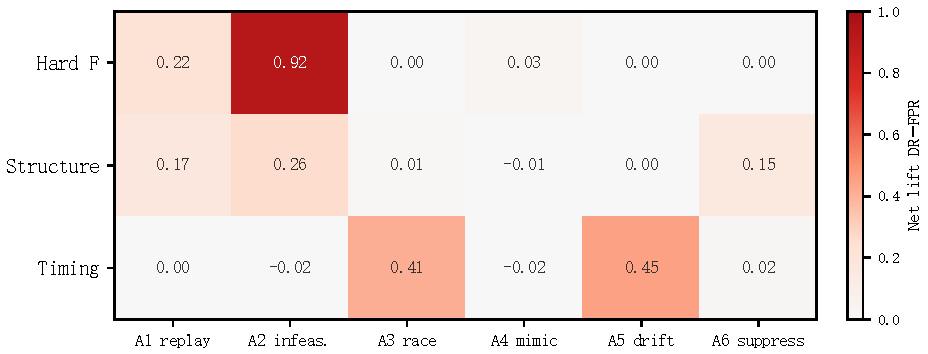
\includegraphics[width=0.98\linewidth]{figures/fig_coverage.pdf}
\caption{三路生产通道相对良性误报的净提升（{DR}$-${FPR}）。{A2} 由硬层覆盖，{A3}/{A5} 仅时序有实质提升，{A4} 没有独占通道。}
\label{fig:coverage}
\Description{三行六列热图：硬层、结构、时序对 A1 至 A6 的净检出提升，A2 硬层与 A3、A5 时序为深色高值，A4 接近零。}
\end{figure}

\subsection{检测问题}
\label{sec:detproblem}

\begin{problem}[调度层注入检测]
\label{prob:detect}
给定仅含正常运行的历史日志、参考过程模型以及用户指定的误报预算 $\alpha$，对在线消息流逐条输出告警，使得纯良性流上的经验误报不超过 $\alpha$，并在延迟预算内检出 {A1}--{A6} 中的注入。检测器不得使用攻击标签调阈值。
\end{problem}

主指标是同一 $\alpha$ 下、延迟预算内的净检出率（扣除偶然地板，见第~\ref{sec:e1}~节），以及以消息数计的检测延迟。算力约束是每条消息 $O(1)$。

% ============================================================
%  第 4 章：方法
% ============================================================
\section{检测方法}
\label{sec:framework}

\subsection{总体架构}
\label{sec:arch}

生产配置为三路并行，任一触发即告警。硬层良性违反率为零，不消耗共形校准样本；$\alpha/3$ 是三路并集的 {Bonferroni} 划分，因而时序与结构各得 $\alpha/3$。这不是硬层有误报，而是并行 {OR} 的代价：单通道方法独享全部 $\alpha$，三路方法在只有一路有信号的攻击上必然被摊薄。两路统计通道各自校准后经 {CUSUM} 累积。不设跨通道合成路。

离线阶段只用正常日志与参考模型。由 {BPMN} 导出 $\mathbf F$；按设备与操作估计转移与停留时长；留出校准折，用共形预测定出两路统计通道的阈值，并用良性流反解 {CUSUM} 门限，使目标平均误报间隔 $\mathrm{ARL}_0=1/\alpha$。在线阶段对每条消息做常数次查表与对数运算，如图~\ref{fig:arch}。

\begin{figure}[!t]
\centering
\begin{tikzpicture}[
  font=\footnotesize,
  box/.style={draw, rounded corners=1pt, align=center, inner sep=4pt},
  arr/.style={-{Latex}}
]
\node[box] (log) {正常日志};
\node[box, right=0.35cm of log] (bpmn) {BPMN};
\node[box, right=0.35cm of bpmn] (fit) {估计 $\tilde P$、时长核};
\node[box, right=0.35cm of fit] (cal) {共形阈值、CUSUM 门限};
\draw[arr] (log) -- (bpmn);
\draw[arr] (bpmn) -- (fit);
\draw[arr] (fit) -- (cal);
\node[above=0.15cm of fit, font=\small] {离线};
\node[box, fill=black!6, below=1.15cm of log] (msg) {消息 $m_t$};
\node[box, fill=red!8, right=0.3cm of msg] (hard) {硬层 $\mathbf F$\\+ 账本};
\node[box, fill=blue!8, right=0.3cm of hard] (stat) {时序 $z$ / 结构 $\tilde P$};
\node[box, fill=green!8, right=0.3cm of stat] (seq) {CUSUM};
\node[box, right=0.3cm of seq] (out) {告警或\\门控更新};
\draw[arr] (msg) -- (hard);
\draw[arr] (hard) -- (stat);
\draw[arr] (stat) -- (seq);
\draw[arr] (seq) -- (out);
\node[below=0.05cm of stat, font=\small] {在线，$O(1)$；并报警按 $\alpha/3$ 划分};
\end{tikzpicture}
\caption{离线拟合与在线三路并行。硬层在统计通道之前，以免不可行样本污染校准；无互锁统计通道，无跨通道合成。}
\label{fig:arch}
\Description{离线阶段由日志与BPMN估计转移、时长核并校准阈值；在线阶段对每条消息依次做硬层否决、时序与结构打分及CUSUM累积。}
\end{figure}

硬约束必须在最前：零成本、可解释，并避免不可行样本进入后续校准。结构与时序并列而非串联，以便同时覆盖``标签错''与``标签对但时间错''。序列检验在最后，因此两路统计通道必须输出分级分数而不是布尔值。算法~\ref{alg:detect}给出在线路径。

\begin{algorithm}[!t]
\caption{调度层注入的在线检测}
\label{alg:detect}
\begin{algorithmic}[1]
\Require 消息 $m=(d,o,t)$；账本 $\mathcal{L}$；掩码 $\mathbf{F}$；核 $(\tilde P,\mu,\sigma)$；共形阈值与门限 $h$
\Ensure 告警或接受
\If{一元能力、二元可达或命令--响应任一违反}
    \State \textbf{return} 告警（硬层原因）
\EndIf
\State 计算时序残差 $z$ 与结构分数 $\tilde P_{o'\to o}$
\State 对两路分别更新 $S\leftarrow\max(0,\,S+s-c)$
\If{任一路 $S\ge h$}
    \State 复位该路；\textbf{return} 告警
\EndIf
\If{隔离窗口内无告警}
    \State 门控更新 $(\mu,\sigma,\tilde P)$ 并锚定状态
\EndIf
\State \textbf{return} 接受
\end{algorithmic}
\end{algorithm}

\subsection{硬层可行性与命令--响应}
\label{sec:hard}

对消息 $(d,o,t)$，硬层依次检查三项，任一失败立即告警并给出原因。
\begin{enumerate}[leftmargin=1.4em,itemsep=2pt]
\item 一元：$(d,o)$ 是否属于参考模型的能力集。
\item 二元：若同一 $(d,\mathrm{case})$ 存在已确认前驱 $o'$，则 $(o'\to o)$ 是否被 $\mathbf F$ 允许。
\item 因果：该状态上报是否存在前置命令事件。
\end{enumerate}
掩码由随数据集发布的 {BPMN} 自动导出：一元能力集取节点上绑定的设备类型（或资源角色），二元可达由同一工作流内的顺序与网关展开，不手工编转移表。一元检查覆盖全部消息，正常数据上违反率为零。训练折未见的良性组合不能当作异常：其比例远高于 $\alpha$，而参考模型拒绝其中 $0$ 条；具体数字见第~\ref{sec:e1}~节。

\subsection{结构通道}
\label{sec:struct}

结构通道询问：当前活动在 case 级工作流序列上是否常见。链粒度取 case 而不是 $(d,\mathrm{case})$：在服务端点型产线上，设备级链大量长度为~$1$，转移概率没有可分的取值。状态是操作名。转移用 {Dirichlet} 后验预测 $\tilde P$，以避免小样本伪零，同时保留 $\mathbf F$ 强制的真零。

交给共形校准器的是预测概率 $\tilde P_{o'\to o}$，而不是随机化 $p$ 值。随机化是为了在直接与 $\alpha$ 比较时打散原子；喂给校准器时应保留原始分数的次序，并列只在阈值处打破一次。该通道对 {A4}/{A6} 这类改变事件数目的攻击敏感，但在三路均分预算后，其单路功效低于独享 $\alpha$ 的纯马尔可夫检测器---这是多通道的固有代价，见第~\ref{sec:e2}~节。

\subsection{半马尔可夫时序通道}
\label{sec:timing}

半马尔可夫核写作 $Q_{o'o}(\tau)=P_{o'o}F_{o'o}(\tau)$。停留时长按 $(\text{设备},\text{操作})$ 分组，取 $\log\tau\sim\mathcal{N}(\mu,\sigma^2)$。时序本身不是创新点；与计时自动机的差别在于 $F_{o'o}$ 是分布而不是区间守卫，见第~\ref{sec:md}~节。生产配置不把路线协变量写入卖点：在全局样本量加权口径下，条件化仅把 $\sigma$ 从 $0.236$ 降到 $0.228$，端到端无增益。

四种观测对应四个分支。
\begin{itemize}[leftmargin=1.4em,itemsep=2pt]
\item \textbf{状态跳变。} 标准化残差 $z=(\log\tau-\mu)/\sigma$，只做左侧检验（``太快''即抢跑）。抢跑是有方向的备择；单侧的价值主要是阈值稳定，而不是功效翻倍。
\item \textbf{同状态心跳。} 右删失生存函数 $-\log\bigl(1-F(\tau)\bigr)$，只在``待太久''时报警。
\item \textbf{超时无消息。} 同一生存函数，由看门狗在高分位触发。它覆盖``活动已开始、完成事件被抑制''，覆盖不到``整条活动从未开始''---后者需要活动间隔模型，本文不提供。
\item \textbf{周期轮询。} 区间删失 $\log\bigl[F(\tau+\Delta)-F(\tau)\bigr]$，以免量化误差污染似然。主实验为事件驱动日志，该分支不参与评测。
\end{itemize}
不符合度分数取 $z$ 本身，不取参数化 $p$ 值。人工工位的 $\sigma$ 可接近~$2$，时序通道在那些分组上接近失效；检测能力由最易变工序决定。

\subsection{共形校准与序贯累积}
\label{sec:conformal}

两路统计通道在留出的正常样本上做分割共形预测~\cite{shafer2008conformal}，经验分位数给出无分布 $\mathrm{FPR}\le\alpha/3$ 的阈值。该保证不依赖高斯或马尔可夫假设成立，但依赖校准集与部署数据可交换。工作流间转移集合的 {Jaccard} 重合度中位数约为 $0.32$，故新产品型号必须重新校准或按型号分层。本日志校准集 $n_{\mathrm{cal}}=701$，可信支撑的最低单消息 $\alpha$ 约为 $10^{-2}$；更低的误报预算由 {CUSUM} 的 $\mathrm{ARL}_0$ 承担。

对各通道的不符合度分数做单侧 {CUSUM}~\cite{li2015quickest}
\begin{equation}
  S_t=\max\bigl(0,\,S_{t-1}+s_t-c\bigr),
  \label{eq:cusum}
\end{equation}
越过门限 $h$ 则告警并复位。$h$ 由良性流标定，目标 $\mathrm{ARL}_0=1/\alpha$。设计位移取 $1\sigma$。告警后必须复位，否则统计量停在门限上方，后续每条都告警。基线中凡输出分级分数的方法套用同一套累积，以免把增益误归因到 {CUSUM} 本身。

\subsection{门控更新与复杂度}
\label{sec:online}

正常消息用于锚定状态，并用指数滑动平均缓慢更新 $(\mu,\sigma)$ 与 $\tilde P$。更新必须门控：仅当该消息通过全部通道、且隔离窗口内无告警时才进入基线。否则攻击者可以用持续的小幅抢跑把时长基线拖向自己，使后续注入逐渐合法化。在持续抢跑下，关闭门控后攻击者可稳定获取的调度提前量约为 $26\%$，门控后降到约 $1\%$。

每条消息 $O(1)$：常数次查表、对数与硬层判断，与状态数、设备数在热路径上无关。多设备可按链并行。第~\ref{sec:e8}~节给出常数因子。

% ============================================================
%  第 5 章：理论分析
% ============================================================
\section{理论分析}
\label{sec:theory}

\subsection{分布型时长与时钟守卫}
\label{sec:md}

计时自动机对转移 $(o',o)$ 给出时钟守卫 $[\ell,u]$：$\tau\in[\ell,u]$ 则接受，否则拒绝~\cite{maier2011timed,lin2018tabor}。设正常停留均值为 $\mu$。若攻击者取抢跑量 $\rho$，使 $(1-\rho)\mu\in[\ell,u]$，则该观测在守卫内，单步判决为正常。守卫是二值的，同一方向上多次略快的停留不会被累积。

半马尔可夫通道输出的是分级残差 $z=(\log\tau-\mu)/\sigma$。抢跑使 $\mathbb{E}[z]=\log(1-\rho)/\sigma<0$。只要该期望低于 {CUSUM} 的参考值，随机游程即以正漂移越过 $h$，即使每条 $|z|$ 都小于单消息共形阈值。这不是停留时长建模本身的新颖性，而是\emph{证据形态}的差别：区间守卫把落在内侧的抢跑映射为零，分布型残差把它映射为可加的增量。图~\ref{fig:guard}给出示意：全部观测落在守卫内，二值通道不报警，{CUSUM} 仍越过门限。{A3} 正落在这一差别上---标签完全合法，计时自动机可以接受，序贯半马尔可夫仍可能检出。

\begin{figure}[!t]
\centering
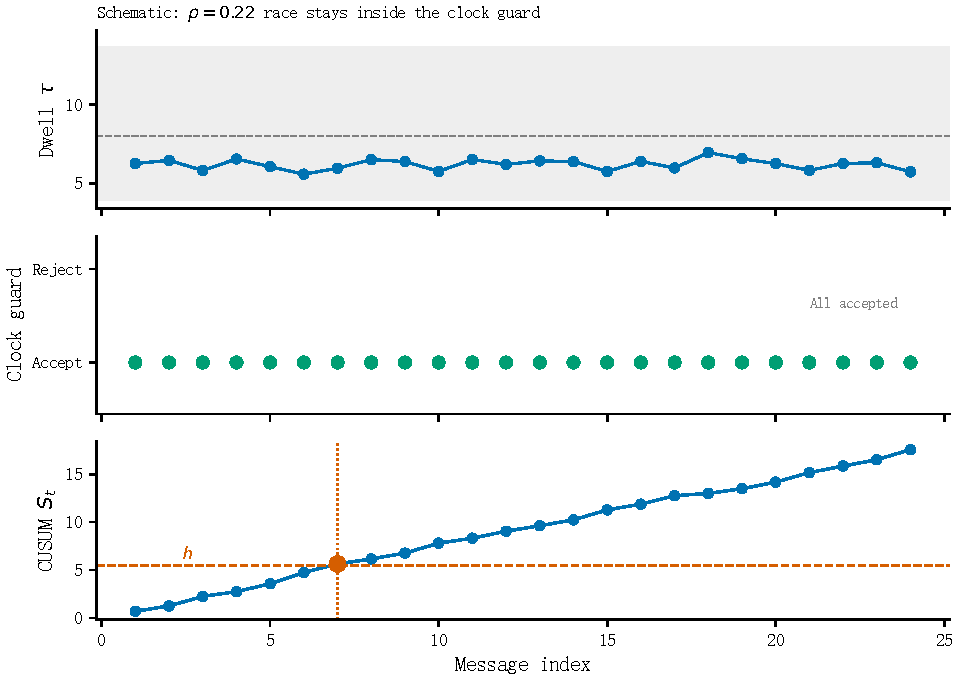
\includegraphics[width=0.95\linewidth]{figures/fig_guard_cusum.pdf}
\caption{时钟守卫与分布型残差的差别（示意，非评测轨迹）。灰色带为区间守卫；同向抢跑全部被接受，{CUSUM} 仍累积越过 $h$。}
\label{fig:guard}
\Description{三行示意：停留时长均落在灰色守卫带内，时钟守卫全部接受，CUSUM 统计量随后越过门限。}
\end{figure}

\subsection{规避检测的抢跑量上界}
\label{sec:bound}

\begin{proposition}[规避检测的抢跑量上界]
\label{prop:rho}
设正常停留满足 $\log\tau\sim\mathcal{N}(\mu,\sigma^2)$，左侧水平为 $\alpha$，阈值为 $-z_{1-\alpha}$。攻击将观测时长缩为 $(1-\rho)\tau$。使攻击后残差均值恰好落在阈值上的抢跑量为
\begin{equation}
  \rho^*(\alpha,\sigma)=1-e^{-\sigma z_{1-\alpha}}.
  \label{eq:rho}
\end{equation}
$k$ 次独立重复下，均值标准差按 $1/\sqrt{k}$ 收缩，
\begin{equation}
  \rho^*_k(\alpha,\sigma)\approx 1-e^{-\sigma z_{1-\alpha}/\sqrt{k}}.
  \label{eq:rhok}
\end{equation}
\end{proposition}

\begin{proof}
对数域位移 $\Delta=\log(1-\rho)$，标准化后均值移动 $\Delta/\sigma$。令 $\Delta/\sigma=-z_{1-\alpha}$，解出 $\rho=1-e^{-\sigma z_{1-\alpha}}$。$k$ 次独立平均把 $\sigma$ 换成 $\sigma/\sqrt{k}$，即得式~\eqref{eq:rhok}。
\end{proof}

式~\eqref{eq:rho}只含时序变异、误报预算与重复次数，不含系统矩阵。它是隐蔽攻击基本极限~\cite{liu2022limits}在离散事件上的实例：体裁不新，实例是抢跑量而不是连续状态的偏差能量。对\emph{单一}高斯，均值落在阈值上对应单消息检出率约 $1/2$。产线工序的 $\sigma$ 高度异质，低变异分组会远早于全局 $\rho^*$ 被抓住，因而\emph{混合}功效曲线在 $\rho<\rho^*$ 时就可以明显高于 $1/2$；第~\ref{sec:e4}~节验证的是这条混合曲线与实测的吻合，而不是``过了 $\rho^*$ 才到半数''。图~\ref{fig:sigma}画出 $\rho^*(\sigma)$：全局 $\sigma=0.236$ 对应 $42.2\%$；人工工位 $\sigma$ 接近 $2$ 时上界失效，产线整体可检测性由最弱环节决定。

\begin{figure}[!t]
\centering
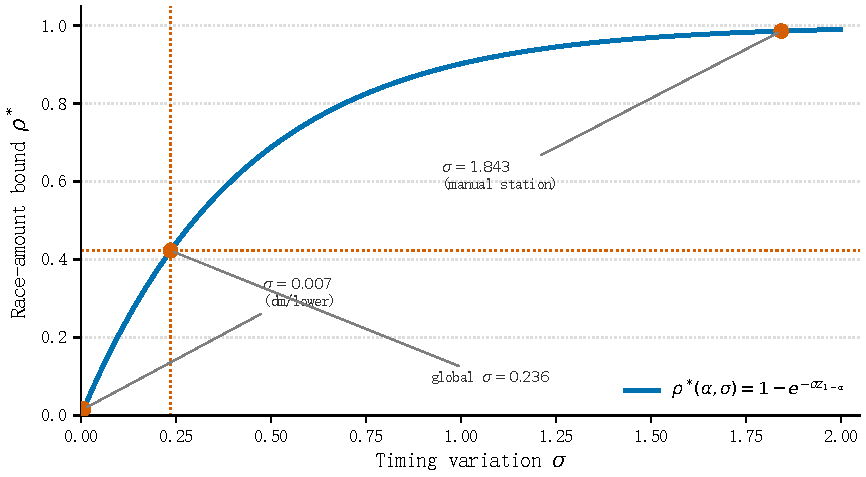
\includegraphics[width=0.82\linewidth]{figures/fig_sigma.pdf}
\caption{$\alpha=0.01$ 单侧下 $\rho^*$ 随 $\sigma$ 的变化。标注点为低变异工序、全局加权 $\sigma$ 与人工工位。}
\label{fig:sigma}
\Description{抢跑量上界随时序变异增大并趋近于一，全局 sigma 为 0.236 时上界约百分之四十二。}
\end{figure}

% ============================================================
%  第 6 章：实验
% ============================================================
\section{实验评估}
\label{sec:experiments}

\subsection{设置}
\label{sec:setup}

主数据集是特里尔大学教学工厂的 Fischertechnik 智能工厂 {IoT} 事件日志~\cite{malburg2022trier}。产线含高架仓库、真空搬运、分拣、铣削、钻孔、冲压、烤炉与人工工位等十余台资源，两条线经工件交换互联。设备是被调度器调用的服务端点：每个作业通常只被调用一到两次，按设备切开的状态链多数长度为~$1$，因此结构通道必须走 case 级工作流链，而不是 $(d,\mathrm{case})$。活动带指派--执行--完成的生命周期，可与命令账本配对。随数据发布 $16$ 个 {BPMN}：一元能力取节点绑定的设备类型（或资源角色），二元可达取同一工作流内顺序与网关的传递闭包，从而自动得到 $\mathbf F$，不手工编转移表。清洗后全日志 $3{,}062$ 条活动。划分按时间序：拟合、校准、测试互不重叠；测试折良性消息 $508$ 条，校准折 $n_{\mathrm{cal}}=701$。注入在测试折上进行，注入率 $20\%$，抢跑默认 $\rho=0.30$，三个随机种子。{A4} 的攻击者按转移模型选择最可能的下一步（知模型），而不是复制当前操作。

主基线三项，均在同一良性参照流上把经验误报对齐到 $\alpha$，并给输出分级分数的方法套上同一套 {CUSUM}（延迟预算 $10$ 条，告警后复位）。
\begin{itemize}[leftmargin=1.4em,itemsep=2pt]
\item {B3}：学习型计时自动机（Maier/{BUTLA} 式），时钟守卫加人工容差~\cite{maier2011timed}。
\item {B4}：{TABOR} 式，计时自动机加站内依赖~\cite{lin2018tabor}。
\item {B5}：显式时长隐半马尔可夫似然~\cite{tan2008hsmm}，观测为操作符号与对数时长，隐状态数由留出似然在 $\{2,3,4,6\}$ 中取 $K=6$。
\end{itemize}
仅标签的一阶马尔可夫似然作为消融对照（记为仅标签），不是独立先行方法：它用于展示去掉时间维之后 {A3}/{A5} 的结构性失明。阈值一律定在同一批 case 的未注入版本上，不用受攻击流内部的``良性''消息---原地改写会让后继良性消息与伪造前驱比对，产生攻击引起的级联触发。

延迟预算内``窗口中任一告警即检出''存在偶然地板 $1-(1-\mathrm{FPR})^{B+1}$（$B=10$）。表中主结果已减去该地板；未减地板的数字不单独引用。逐消息检出受参照流长度限制，本规模下不作主结果。

\subsection{与计时自动机及半马尔可夫的对照}
\label{sec:e1}

表~\ref{tab:e1}是 $\alpha=0.01$ 下的净检出率。本方法均值为 $0.48$，{B3}/{B4}/{B5} 为 $0.17/0.21/0.11$。主张不写成全面优于，而写成三句。第一，{A3}/{A5} 是纯时序攻击，标签未改；仅标签消融减地板后为 $-0.01$ 与 $0.00$，即分数流与良性流逐条相同。本方法为 $0.18$ 与 $0.87$。{B3}/{B4} 在 {A3} 上只有 $0.10$，与区间守卫接受内侧抢跑相一致；{A5} 上计时自动机有累积式漂移可抓（$0.59/0.48$），仍低于分布型通道。{B5} 在 {A3} 上仅 $0.06$，是因为其时长核绑在隐状态上，而不是按 $(\text{设备},\text{操作})$ 做左尾检验：标签未改的抢跑被吸收为``该隐状态一次略短的停留''，似然下降不足以在 $\alpha$ 下越界。第二，{A1}/{A2} 上本方法为 $0.55/0.95$，高于三条主基线；{A2} 由硬层覆盖，{B4} 的站内依赖不能替代参考模型。第三，{A4}/{A6} 上本方法为 $0.17/0.14$，低于仅标签消融的 $0.23/0.28$---三路均分使结构通道只得 $\alpha/3$，而这两类攻击主要改变事件数目。这是多通道方法的预算代价，不是通道设计失败。表~\ref{tab:coverage}是单通道、单消息、未减地板的覆盖诊断；表~\ref{tab:e1}是三路并行、延迟预算 $10$、已减偶然地板的端到端净检出。因此 {A3} 时序单消息 $0.43$ 与表~\ref{tab:e1}的 $0.18$ 并不矛盾：后者把预算摊到 $\alpha/3$，再减去窗口偶然地板。

\begin{table}[!t]
\renewcommand{\arraystretch}{1.15}
\caption{$\alpha=0.01$、延迟预算 $10$ 条、已减偶然地板的净检出率。仅标签为马尔可夫消融。序贯误报（名义 $0.01$）依次为 $0.006$、$0.006$、$0.008$、$0.004$（仅标签 $0.008$）。}
\label{tab:e1}
\centering
\small
\begin{tabular}{lccccc}
\toprule
攻击 & {B3} {BUTLA} & {B4} {TABOR} 式 & {B5} {HSMM} & 仅标签 & 本文 \\
\midrule
{A1} 朴素重放 & $0.04$ & $0.04$ & $-0.01$ & $0.48$ & $0.55$ \\
{A2} 不可行注入 & $0.37$ & $0.67$ & $0.31$ & $0.76$ & $0.95$ \\
{A3} 抢跑重放 & $0.10$ & $0.10$ & $0.06$ & $-0.01$ & $0.18$ \\
{A4} 状态模仿 & $-0.04$ & $-0.01$ & $0.02$ & $0.23$ & $0.17$ \\
{A5} 渐变漂移 & $0.59$ & $0.48$ & $0.25$ & $0.00$ & $0.87$ \\
{A6} 消息抑制 & $-0.05$ & $-0.01$ & $0.05$ & $0.28$ & $0.14$ \\
\midrule
均值 & $0.17$ & $0.21$ & $0.11$ & $0.29$ & $0.48$ \\
\bottomrule
\end{tabular}
\end{table}

图~\ref{fig:e1}把表~\ref{tab:e1}画成柱状对照。仅标签消融在 {A3}/{A5} 上贴着零线，是去掉时间维后的结构性失明；本文在 {A4}/{A6} 上低于该消融，与三路均分预算一致，并不改写为全面优于。

\begin{figure}[!t]
\centering
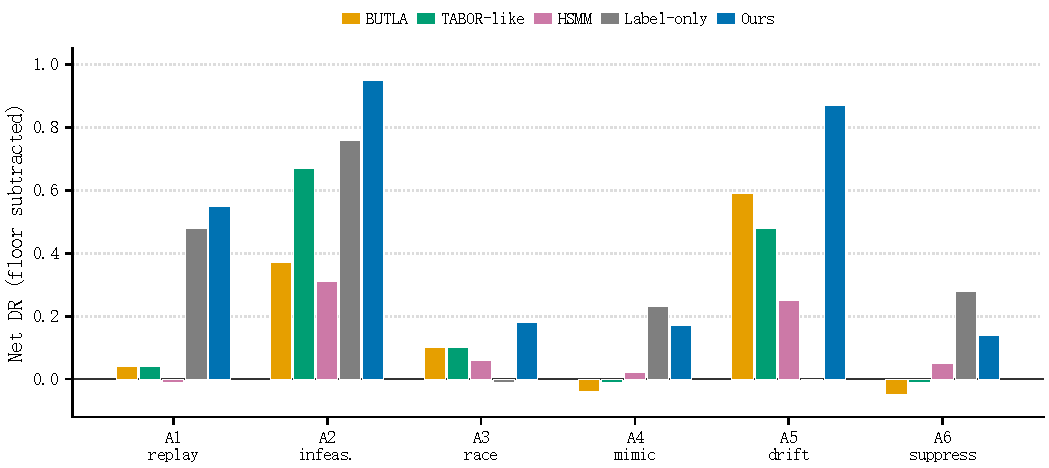
\includegraphics[width=0.98\linewidth]{figures/fig_e1_dr.pdf}
\caption{$\alpha=0.01$、延迟预算 $10$ 条、已减偶然地板的净检出率。仅标签为马尔可夫消融，不是独立先行方法。}
\label{fig:e1}
\Description{六类攻击上 BUTLA、TABOR 式、HSMM、仅标签与本文的分组柱状图，本文在 A2 与 A5 最高，仅标签在 A3 与 A5 为零。}
\end{figure}

{B4} 与 {B3} 在多格上接近：站内依赖在本日志上信息量低，且给``该设备从未做过此操作''的极端分数已在良性测试折出现（即上述 $3.9\%$ 未见组合）。参考模型拒绝这 $20$ 条中的 $0$ 条。{B5} 的 {EM} 似然单调收敛，时长核非退化，是与时序加结构对位的基线；均值 $0.11$，说明把状态当作隐变量并没有自动获得可行性掩码。按校准折定阈值后在测试折的误报：{B3}/{B4} 为名义值的 $3.7$ 倍，{B5} 为 $1.0$ 倍。共形的对照因此不是``只有本文控得住误报''，而是控制不依赖模型假设成立。$\alpha=0.05$ 下各格排序不变，{A4}/{A6} 的落后不是分辨率假象。

\subsection{消融}
\label{sec:e2}

消融在 $\alpha=0.05$、\emph{每路误报预算固定}的设置下进行，以避免``去掉一路等于给其余路加预算''的混淆。完整配置六族均值为 $0.41$。去掉时序通道后均值下降 $0.11$，且 {A3}/{A5} 精确归零（$0.27\to 0.01$，$0.70\to -0.02$）。这与表~\ref{tab:e1}中仅标签消融在同两格上的零是同一现象的两个独立证据。去掉硬层后均值下降 $0.07$，集中在 {A2} 与 {A1}。去掉结构通道后均值下降 $0.04$，集中在 {A4} 与 {A6}。图~\ref{fig:e2}给出按攻击族的对照与均值变化。

\begin{figure}[!t]
\centering
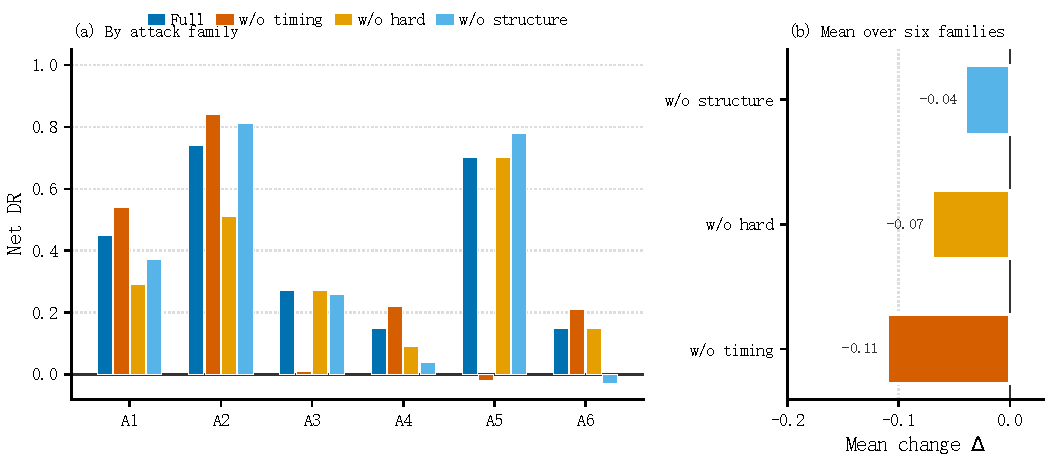
\includegraphics[width=0.98\linewidth]{figures/fig_e2_ablation.pdf}
\caption{生产三路的消融（每路误报预算固定，$\alpha=0.05$）。去掉时序后 {A3}/{A5} 归零；硬层与结构的贡献分别集中在 {A2}/{A1} 与 {A4}/{A6}。}
\label{fig:e2}
\Description{左图为完整、去时序、去硬层、去结构在六类攻击上的柱状对照；右图为均值下降 0.11、0.07、0.04。}
\end{figure}

共形在检出率口径上接近于零（$-0.01$），因为它的作用是把误报对齐；其证据在误报侧：参数阈值会使经验误报接近翻倍。物料令牌不变量与跨通道合成路曾作为候选统计通道，在良性发生率天花板与端到端消融上净贡献为非正，不进入生产配置，也不占 $\alpha$ 预算。

\subsection{抢跑量与理论界}
\label{sec:e4}

在真实时长上注入 $\tau\mapsto(1-\rho)\tau$。命题~\ref{prop:rho}的 $\rho^*$ 使用全局拟合折 $\sigma=0.236$（不用协变量口径）；$\alpha=0.01$ 单侧时 $\rho^*=42.2\%$。表~\ref{tab:e4}与图~\ref{fig:e4}的理论列是按工序分组后的混合预测，不是把全局 $\sigma$ 代入单一高斯后、在 $\rho^*$ 处应等于 $1/2$ 的那一点：$\rho=0.30<\rho^*$ 时实测单消息检出 $0.45$，在 $\rho=0.40\approx\rho^*$ 时为 $0.71$。全区间平均绝对偏差约 $0.03$。{CUSUM} 把弱信号变成可用检测：$\rho=0.15$ 时单消息检出 $0.20$，累积后 $0.87$，中位延迟 $10$ 条消息；$\rho=0.30$ 时中位延迟 $4$ 条，见图~\ref{fig:delay}。检出率在约 $0.96$ 处饱和，剩余来自 $\sigma$ 极大的分组，与``最弱环节''陈述一致。

\begin{table}[!t]
\renewcommand{\arraystretch}{1.12}
\caption{$\alpha=0.01$ 单侧下抢跑量扫描。位移 $\Delta=\log(1-\rho)$；理论列为按工序混合后的预测，不是全局 $\sigma$ 下单一高斯在 $\rho^*$ 处的 $1/2$ 点。}
\label{tab:e4}
\centering
\small
\begin{tabular}{ccccc}
\toprule
$\rho$ & $\lvert\Delta\rvert$ & $\lvert\Delta\rvert/\bar\sigma$ & 实测 {DR} & 理论 \\
\midrule
$0.05$ & $0.051$ & $0.21$ & $0.060$ & $0.051$ \\
$0.10$ & $0.105$ & $0.44$ & $0.105$ & $0.127$ \\
$0.15$ & $0.163$ & $0.68$ & $0.199$ & $0.226$ \\
$0.20$ & $0.223$ & $0.93$ & $0.288$ & $0.317$ \\
$0.30$ & $0.357$ & $1.49$ & $0.452$ & $0.497$ \\
$0.40$ & $0.511$ & $2.14$ & $0.712$ & $0.701$ \\
$0.50$ & $0.693$ & $2.90$ & $0.874$ & $0.851$ \\
\bottomrule
\end{tabular}
\end{table}

\begin{figure}[!t]
\centering
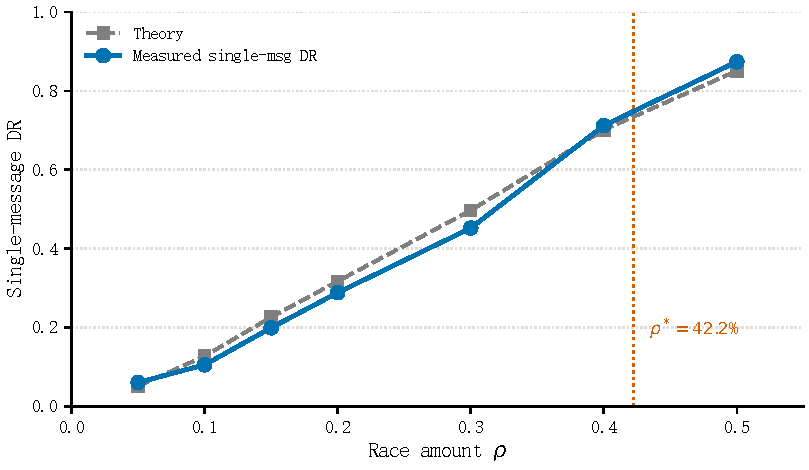
\includegraphics[width=0.82\linewidth]{figures/fig_e4_rho.pdf}
\caption{单消息检出率随抢跑量的变化。理论列为分组混合预测；竖线为全局 $\sigma=0.236$ 下的 $\rho^*=42.2\%$。}
\label{fig:e4}
\Description{实测单消息检出率与按工序混合的理论预测随抢跑量上升；竖线标出全局 sigma 下的 rho 星，该处混合功效已明显高于二分之一。}
\end{figure}

\begin{figure}[!t]
\centering
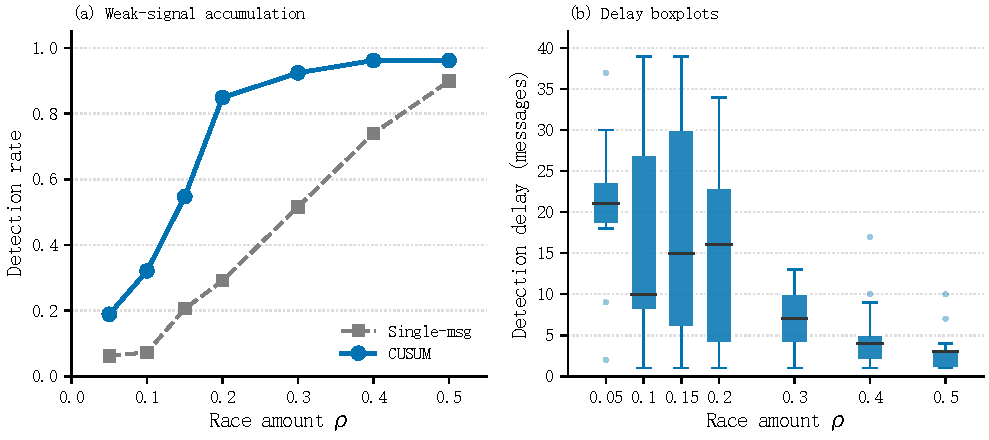
\includegraphics[width=0.98\linewidth]{figures/fig_delay.pdf}
\caption{{CUSUM} 相对单消息阈值的功效与检测延迟。延迟为中位数，上须为 $p_{90}$；无逐次分位存档，故不作箱线图。}
\label{fig:delay}
\Description{左图 CUSUM 检出率在小抢跑量下明显高于单消息；右图中位延迟随抢跑量下降。}
\end{figure}

\subsection{处理时延}
\label{sec:e8}

单核逐消息时延中位 $81\,\mu\mathrm{s}$，{$p_{95}=116\,\mu\mathrm{s}$}，{$p_{99}=159\,\mu\mathrm{s}$}，等效吞吐约 $1.23\times 10^{4}$ 条/秒，见图~\ref{fig:latency}。相对本日志的活动到达间隔，余量在三个数量级以上。未做专用工业控制器实测；``边缘可部署''由 $O(1)$ 热路径加上上述常数因子支撑。

\begin{figure}[!t]
\centering
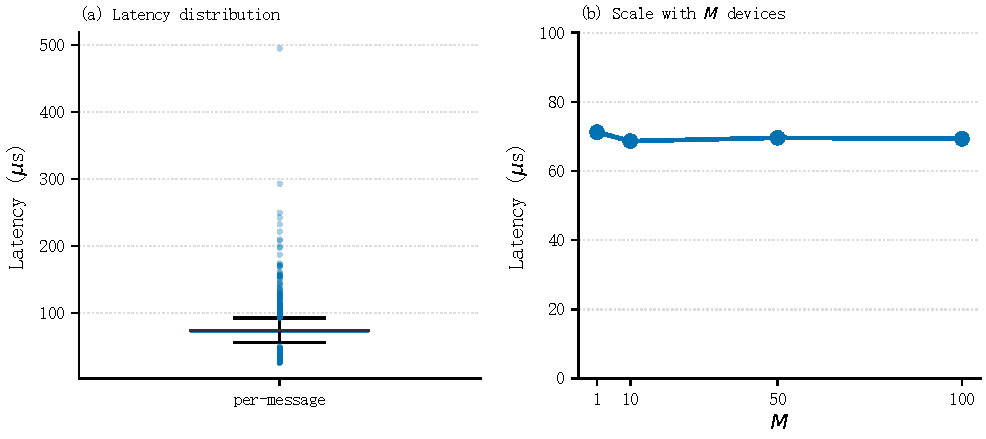
\includegraphics[width=0.48\linewidth]{figures/fig_latency.pdf}
\caption{单核逐消息处理时延。中位 $81\,\mu\mathrm{s}$，$p_{95}=116\,\mu\mathrm{s}$，$p_{99}=159\,\mu\mathrm{s}$。}
\label{fig:latency}
\Description{三条柱分别给出逐消息处理时延的中位、百分之九十五与百分之九十九分位。}
\end{figure}

% ============================================================
%  第 7 章：结论
% ============================================================
\section{结论}
\label{sec:conclusion}

本文将生产调度层的注入攻击检测表述为独立问题：对象是调度器对离散状态标签的信任，而不是连续控制或报文会话。方法上，参考模型可行性掩码与命令账本构成硬层，半马尔可夫停留核与 case 级结构通道在指定误报预算下并行累积。相对分解式计时自动机与站内依赖模型，可辩护的差别是两点：分布型时长使守卫内侧的抢跑可被累积；可行性不能从日志学出，必须外挂参考模型。规避检测的抢跑量被 $\rho^*(\alpha,\sigma)$ 封顶，并在产线日志上与实测检出率吻合。

局限如下。第一，状态模仿与整段活动抑制在生产配置下没有独占通道，且在 {A4}/{A6} 上低于仅标签检测器，代价来自多路预算摊薄。第二，物料流不变量在缺少工件身份时良性违反率使统计功效被封顶，不能作为现行通道。第三，多设备协同伪造超出声明范围，未实现即不报告。第四，跨域的周期轮询日志尚未评测；共形保证在产品型号切换时要求重新校准。后续工作应在带工件标识的产线上重新检验令牌约束能否升为硬层，并把 $\alpha$ 在连续通道之间的分配写成不依赖攻击标签的规则。

% Bibliography (placed at document end)
\bibliographystyle{ACM-Reference-Format}
\bibliography{reference-base}

\end{document}